\section{Dataset}\label{sec:dataset}

Using \tcpsnitchns, we recorded traces for 90 Android and 33 Linux
applications by manually interacting with each application for a few seconds
in order to reproduce a typical usage. We mainly selected popular
consumer-oriented client applications and the dataset currently does not
include any server-side application. For some popular applications, we recorded
multiple traces in different network environments.

We observed major differences in the API usage patterns on Android and Linux.
For instance, the most popular API functions differ and applications use
different recurring combinations of socket options. In accordance with
\cite{Atlidakis:POSIX}, we confirm that high-level frameworks and libraries
drive the API usage and are at the root of such glaring
disparities. Due to space limitations, we restrict our analysis to the
Android dataset for the rest of this paper. The full dataset with
various visualizations is publicly available from \url{https://tcpsnitch.org}.

Our Android dataset mostly includes highly popular applications from different
categories of apps in the Google Play Store. Table~\ref{tab:apps} shows a
sample of representative applications. At the time of writing, all Android
traces have been recorded on Android 6.0.1 with a LG Nexus 5 device.
In total, the Android dataset includes 181 application traces
that opened a total of 16.384 sockets. This represents about 2.3M intercepted
function calls.

\begin{table}[]
    \centering
    \begin{tabular}{ll}
        \hline
        \multicolumn{1}{|l|}{\textbf{Category}} & \multicolumn{1}{l|}{\textbf{Applications}} \\ \hline
        Social                                  & Facebook, Twitter, Linkedin                \\
        Streaming                               & Spotify, Netflix, Soundcloud               \\
        Video-telephony                         & Skype, Viber, Hangout                      \\
        Shopping                                & Amazon, AliExpress,  Zalando               \\
        Browsers                                & Chrome, Firefox, Opera                     \\
        Productivity                            & Evernote, Slack, Mega                      \\
        Video/photo                             & Youtube, Instagram, Pinterest
    \end{tabular}
    \caption{Sample applications. \textmd{The Android dataset contains traces
of 90 applications from different categories of apps in the Google Play Store.}}
    \label{tab:apps}
\end{table}

\subsection{Usage of the socket API functions}

The socket API contains various functions that often have overlapping
purposes. For instance, there are as many as 7 functions to send data:
\texttt{write()}, \texttt{send()}, \texttt{sendto()}, \texttt{writev()},
\texttt{sendmsg()},\texttt{sendmmsg()} and\\\texttt{sendfile()}.
Figure~\ref{fig:functions_usage} shows the number of applications using
each intercepted function. This section intends to
shed some light about the real usage of these functions.

Some functions are used by a large fraction of the applications. For instance,
\texttt{getsockopt()}, \texttt{setsockopt()} and \texttt{fnctl()}
are used by all the applications in our dataset and only one
application does not call \texttt{get\-sock\-name()}. Another surprising result
is that a textbook server-side function such as
\texttt{bind()} is used by 96\% of our client Android
applications.  We observe that about 95\% of
these \texttt{bind()} calls specify \texttt{INADDR\_ANY} as the IP address and
0 for the port number (meaning an OS assigned random port) but explicitly request
for an IPv6 address. This usage is mainly driven by the \texttt{Socket} class
of the Android SDK~\cite{aosp_socket} that caches the local address of the
socket (using \texttt{get\-sock\-name()}) before trying to connect it.

\begin{figure}
\centering
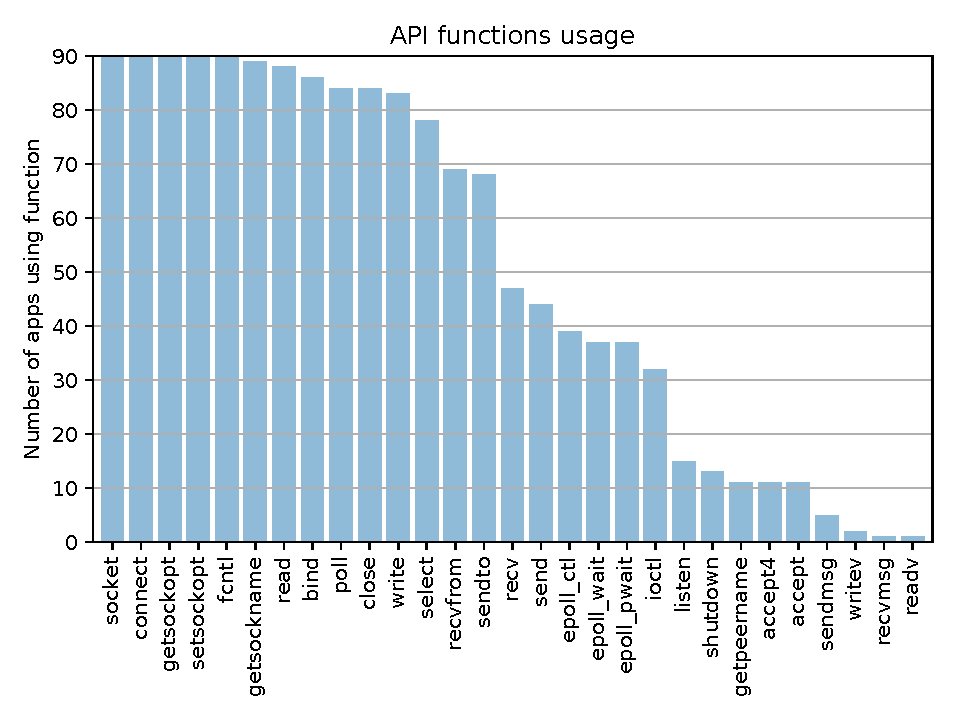
\includegraphics[width=\columnwidth]{figures/functions_bars}
\caption{API functions usage. \textmd{A dozen API functions are used by almost
all applications. Vectored I/O functions are mostly unused.}}
\label{fig:functions_usage}
\end{figure}

Some of our observations are dependent on Android 6.0.1. For instance,
Bionic, Google's implementation of \texttt{libc},
implements some API functions by calling their more complex sibling,
e.g. \texttt{send()} is implemented by calling \texttt{sendto()}. When the
simple version of these 'twin' functions \footnote{Here is a complete list of
these twin functions: \texttt{send()} calls \texttt{sendto()}, \texttt{recv()}
calls \texttt{recvfrom()}, \texttt{accept()} calls \texttt{accept4()} and
\texttt{epoll\_wait} calls \texttt{epoll\_pwait()}.} is called, \tcpsnitch
records 2 consecutive function calls although the application code actually
performs a single function call. This means that the popularity of
\texttt{sendto()}, \texttt{recvfrom()}, \texttt{accept4()} and
\texttt{epoll\_pwait()} is overestimated on Fig.~\ref{fig:functions_usage}.

We did not observe any utilization of \texttt{sendfile()}, \texttt{sendmmsg()}
and \texttt{recvmmsg()}. These 3 functions are optimizations
mostly useful for server-side applications requiring high-performance.
For instance, \texttt{sendfile()} is a Linux specific call that saves 
a back-and-forth copy between kernel
and user space when sending a file over a socket, while \texttt{sendmmsg()} and
\texttt{recvmmsg()} allow to send or receive multiple \texttt{struct msghdr}
in a single system call.

Figure~\ref{fig:functions_usage} also shows that vectored I/O functions such as
\texttt{readv()} and \texttt{recvmsg()} are seldom used an Android.

\subsection{Types of sockets}

In the IPv6 enabled WiFi network used for the experiments, all but one application
established a TCP connection with a remote host over IPv6. This is a
confirmation of the growing importance of IPv6. All the surveyed
applications opened at least one IPv6 socket while only 64\% opened an IPv4
socket.

While all applications use asynchronous sockets, a single application used the
\texttt{SOCK\_NONBLOCK} optional flag when calling \texttt{socket()}.
\texttt{SOCK\_CLOEXEC} was never used. Most sockets are made asynchronous after
their creation using \texttt{fcntl(F\_SETFL)} and 5 applications used
\texttt{ioctl(FIONBIO)}. Usually, TCP sockets are turned asynchronous just
before the \texttt{connect()} call. As a matter a fact, \texttt{O\_NONBLOCK} is
the only file status flag used by the studied Android applications with
\texttt{fnctl(F\_SETFL)} and \texttt{fnctl(F\_GETFL)}. The \texttt{O\_APPEND},
\texttt{O\_ASYNC}, \texttt{O\_DIRECT} and \texttt{O\_NOATIME} flags were never
used.
